\documentclass[11pt, a4paper]{report}

% --- CÀI ĐẶT UNIVERSAL PREAMBLE ---
% Gói này rất quan trọng để hỗ trợ tiếng Việt
\usepackage{fontspec} % Cho phép chọn font
\usepackage{polyglossia}
\setdefaultlanguage{vietnamese}

% Cấu hình lề giấy
\usepackage[a4paper, top=2.5cm, bottom=2.5cm, left=2.5cm, right=2.5cm]{geometry}

\usepackage{array}
\usepackage{longtable}
% \usepackage{geometry} % Đã định nghĩa ở trên, có thể bỏ dòng này
% \geometry{a4paper, margin=1in} % Đã định nghĩa ở trên, có thể bỏ dòng này
\usepackage{booktabs} % Cho toprule, midrule, bottomrule
\usepackage{amsmath} % Gói toán học cơ bản, đôi khi cần cho các ký tự
\usepackage{amsfonts}
\usepackage{amssymb}
\usepackage{enumitem} % Để tùy chỉnh list (gạch đầu dòng)
\usepackage{float}    % Để tùy chỉnh vị trí hình ảnh và bảng

% Chọn font Times New Roman cho chữ chính và JetBrains Mono cho code
\setmainfont{Times New Roman}
\setmonofont{JetBrains Mono}[Scale=0.9]

% Định nghĩa font riêng cho listings
\newfontfamily\listingsfont{JetBrains Mono}[Scale=0.9]

% Sửa lỗi hiển thị gạch đầu dòng (list bullets)
% \setlist[itemize]{label=-} % Lỗi này thường không xảy ra với polyglossia và fontspec, có thể bỏ nếu không cần thiết.

% --- CÁC GÓI BỔ SUNG CHO BÁO CÁO NÀY ---
\usepackage{graphicx}     % Để chèn hình ảnh (biểu đồ)
% \usepackage{booktabs}     % Đã khai báo ở trên
\usepackage{listings}     % Để chèn code Java (bạn sẽ dùng Python)
\usepackage{xcolor}       % Để định nghĩa màu cho code
\usepackage{indentfirst}
\usepackage{titlesec}
% Đặt độ dài thụt lề đầu dòng (15pt là giá trị phổ biến)
\setlength{\parindent}{15pt}
\usepackage[unicode=true]{hyperref} % Để hỗ trợ tiếng Việt trong PDF bookmarks, nên đặt cuối cùng

% Cấu hình màu sắc cho code listing
\definecolor{codegreen}{rgb}{0,0.6,0}
\definecolor{codegray}{rgb}{0.5,0.5,0.5}
\definecolor{codepurple}{rgb}{0.58,0,0.82}
\definecolor{backcolour}{rgb}{0.98,0.98,0.98}

% Cấu hình style cho code Python với XeLaTeX
\lstdefinestyle{mystyle}{
    backgroundcolor=\color{backcolour},
    commentstyle=\color{codegreen},
    keywordstyle=\color{magenta}, % Hoặc màu khác cho Python keywords
    numberstyle=\tiny\color{codegray},
    stringstyle=\color{codepurple},
    basicstyle=\listingsfont\footnotesize,
    breakatwhitespace=false,
    breaklines=true,
    captionpos=b,
    keepspaces=true,
    numbers=left,
    numbersep=5pt,
    showspaces=false,
    showstringspaces=false,
    showtabs=false,
    tabsize=2,
    language=Python % <-- CHỈ ĐỊNH NGÔN NGỮ LẬP TRÌNH LÀ Python
}

% Cấu hình chung cho listings
\lstset{style=mystyle}

% --- BẮT ĐẦU TÀI LIỆU ---
\begin{document}

% --- TRANG BÌA ---
\begin{titlepage}
    \centering
    \sffamily

    {\Large ỦY BAN NHÂN DÂN THÀNH PHỐ HỒ CHÍ MINH\par}
    {\LARGE \textbf{TRƯỜNG ĐẠI HỌC SÀI GÒN}\par}
    {\Large \textbf{KHOA CÔNG NGHỆ THÔNG TIN}\par}
    \vspace{1cm}

    
\includegraphics[width=0.3\textwidth]{images/logo_sgu.png}

    \vfill

    {\Huge \textbf{BÁO CÁO}}\par
    \vspace{0.5cm}
    {\Large HỌC PHẦN: AN TOÀN VÀ BẢO MẬT DỮ LIỆU TRONG HỆ THỐNG THÔNG TIN}\par
    
    \vspace{1cm}
    {\Huge \textbf{PHẦN MỀM QUẢN LÝ MẬT KHẨU AN TOÀN}}\par

    \vfill

    \begin{flushright}
    \large
    \begin{tabular}{ll}
        \textbf{Giảng viên:} & Trương Tấn Khoa \\
        \textbf{Nhóm thực hiện:} & 46 \\
    \end{tabular}
    \end{flushright}

    \vspace{0.5cm}

    \textbf{\large Danh sách thành viên:}\par
    \large Mai Trần Tuấn Kiệt – 3122560038\par

    \vfill

    {\large Thành phố Hồ Chí Minh, tháng 11 năm 2025\par}
\end{titlepage}

% --- ĐÁNH SỐ TRANG RÔ-MA CHO CÁC TRANG MỞ ĐẦU ---
\pagenumbering{roman}
\chapter*{LỜI CẢM ƠN}
\addcontentsline{toc}{chapter}{LỜI CẢM ƠN} % Thêm vào mục lục thủ công

Trong quá trình thực hiện đồ án "Phần mềm quản lý mật khẩu an toàn", tôi đã nhận được sự hướng dẫn tận tình, những ý kiến đóng góp quý báu từ quý Thầy/Cô và sự hỗ trợ không ngừng từ bạn bè, gia đình.

Trước hết, tôi xin gửi lời cảm ơn đến Thầy Trương Tấn Khoa, giảng viên môn An toàn và Bảo mật Dữ liệu trong Hệ thống Thông tin, người đã tận tình truyền đạt kiến thức, hướng dẫn và định hướng cho tôi từ những ý tưởng ban đầu cho đến khi hoàn thiện sản phẩm. Những lời khuyên, sự động viên của Thầy là nguồn động lực to lớn giúp tôi vượt qua những khó khăn trong quá trình nghiên cứu và phát triển.

Tôi cũng xin gửi lời cảm ơn đến Trường Đại học Sài Gòn, Khoa Công nghệ Thông tin đã tạo điều kiện thuận lợi về cơ sở vật chất, tài liệu học tập để tôi có thể hoàn thành đồ án này.

Cuối cùng, tôi xin gửi lời cảm ơn đến gia đình và bạn bè đã luôn ở bên, ủng hộ và động viên tôi trong suốt thời gian thực hiện đồ án.

Xin chân thành cảm ơn!

\vspace{1cm}
\begin{flushright}
\textbf{Sinh viên thực hiện}\par
Mai Trần Tuấn Kiệt\par
\end{flushright}
\newpage % Lời cảm ơn (tùy chọn)
\chapter*{TÓM TẮT}
\addcontentsline{toc}{chapter}{TÓM TẮT} % Thêm vào mục lục thủ công

Đồ án này tập trung vào việc nghiên cứu, thiết kế và triển khai một phần mềm quản lý mật khẩu an toàn mang tên AuraCrypt. Với sự gia tăng của các dịch vụ trực tuyến, việc quản lý và bảo mật một lượng lớn mật khẩu đã trở thành thách thức lớn đối với người dùng. AuraCrypt được phát triển nhằm giải quyết vấn đề này, cung cấp một giải pháp hiệu quả để lưu trữ, mã hóa và quản lý thông tin đăng nhập một cách an toàn trên nhiều nền tảng.

Phần mềm sử dụng thuật toán mã hóa đối xứng tiên tiến AES-256-GCM để bảo vệ toàn bộ dữ liệu người dùng, kết hợp với PBKDF2 để tăng cường độ an toàn cho mật khẩu chủ. Ngoài ra, AuraCrypt tích hợp các tính năng tiện ích như tạo mật khẩu mạnh, quản lý danh mục thông minh, sao lưu tự động và khả năng xuất/nhập dữ liệu. Giao diện người dùng được thiết kế trực quan, thân thiện, giúp người dùng dễ dàng thao tác.

Kết quả của đồ án là một ứng dụng quản lý mật khẩu độc lập trên Windows, đảm bảo tính bảo mật cao và mang lại trải nghiệm người dùng liền mạch, góp phần nâng cao ý thức và hiệu quả bảo mật thông tin cá nhân.

\vspace{1cm}
\begin{flushright}
\textbf{Sinh viên thực hiện}\par
Mai Trần Tuấn Kiệt\par
\end{flushright}
\newpage     % Tóm tắt (Abstract)
% \input{muc_luc}     % Mục lục (nếu muốn một file riêng)
\tableofcontents % Nếu bạn muốn nó tự động tạo, hãy để đây.

\listoffigures % Danh sách hình ảnh (nếu có nhiều hình)
\listoftables  % Danh sách bảng biểu (nếu có nhiều bảng)
\newpage

% --- ĐÁNH SỐ TRANG SỐ CHO NỘI DUNG CHÍNH ---
\pagenumbering{arabic}
\setcounter{page}{1} % Bắt đầu lại số trang từ 1

% --- NẠP CÁC CHƯƠNG TỪ CÁC FILE RIÊNG ---
\chapter{GIỚI THIỆU}
\section{Đặt vấn đề}
Trong thời đại số hóa hiện nay, mỗi cá nhân và tổ chức đều phải quản lý một lượng lớn tài khoản trực tuyến với các mật khẩu khác nhau. Việc sử dụng mật khẩu yếu, trùng lặp hoặc ghi nhớ chúng một cách thủ công không chỉ gây bất tiện mà còn tiềm ẩn nguy cơ bảo mật nghiêm trọng. Các cuộc tấn công mạng, rò rỉ dữ liệu ngày càng phức tạp đã đặt ra yêu cầu cấp thiết về một giải pháp quản lý mật khẩu an toàn và hiệu quả.

\section{Mục tiêu đồ án}
Đồ án "Phần mềm quản lý mật khẩu an toàn AuraCrypt" nhằm đạt được các mục tiêu sau:
\begin{itemize}
    \item Thiết kế và triển khai một ứng dụng quản lý mật khẩu với khả năng mã hóa dữ liệu mạnh mẽ, đảm bảo tính bảo mật và toàn vẹn của thông tin.
    \item Phát triển một giao diện người dùng trực quan, thân thiện, dễ sử dụng cho người dùng cuối.
    \item Tích hợp các tính năng hỗ trợ như tạo mật khẩu mạnh, quản lý danh mục, tìm kiếm nhanh và sao lưu dữ liệu tự động.
    \item Đảm bảo khả năng hoạt động trên nền tảng Windows dưới dạng một ứng dụng độc lập, không yêu cầu cài đặt thêm các thư viện Python.
\end{itemize}

\section{Tổng quan về AuraCrypt}
AuraCrypt là một phần mềm quản lý mật khẩu được phát triển bằng Python sử dụng framework Flet. Phần mềm này cung cấp một kho lưu trữ an toàn cho các thông tin đăng nhập, bảo vệ chúng bằng thuật toán mã hóa AES-256-GCM. Người dùng có thể dễ dàng thêm, sửa, xóa, tìm kiếm và phân loại các mục nhập mật khẩu. AuraCrypt cũng bao gồm các tính năng như tạo mật khẩu ngẫu nhiên, tự động sao lưu dữ liệu và một quy trình thiết lập ban đầu thân thiện với người dùng.

\section{Cấu trúc báo cáo}
Báo cáo này được cấu trúc thành 5 chương chính:
\begin{itemize}
    \item \textbf{Chương 1: Giới thiệu} - Trình bày bối cảnh, đặt vấn đề, mục tiêu và tổng quan về đồ án.
    \item \textbf{Chương 2: Cơ sở lý thuyết} - Tổng hợp các kiến thức nền tảng về mật mã học, thuật toán mã hóa, quản lý mật khẩu và các công nghệ liên quan.
    \item \textbf{Chương 3: Phân tích và thiết kế} - Chi tiết hóa các yêu cầu, phân tích hệ thống, kiến trúc phần mềm và thiết kế giao diện người dùng.
    \item \textbf{Chương 4: Triển khai và thử nghiệm} - Mô tả quá trình hiện thực hóa các tính năng, công nghệ sử dụng và kết quả thử nghiệm.
    \item \textbf{Chương 5: Kết luận và hướng phát triển} - Đánh giá tổng thể đồ án, những hạn chế và các định hướng phát triển trong tương lai.
\end{itemize}
\newpage
\chapter{CƠ SỞ LÝ THUYẾT}

\section{Mật mã học cơ bản}
\subsection{Mã hóa đối xứng (Symmetric-key Cryptography)}
Mã hóa đối xứng là phương pháp mã hóa và giải mã dữ liệu sử dụng cùng một khóa bí mật. Tính đơn giản và tốc độ xử lý nhanh làm cho nó trở thành lựa chọn phổ biến để mã hóa lượng lớn dữ liệu.

\subsection{Thuật toán AES (Advanced Encryption Standard)}
AES là một thuật toán mã hóa khối đối xứng được sử dụng rộng rãi trên toàn thế giới. AES hỗ trợ các kích thước khóa 128, 192, và 256 bit. Trong đồ án này, chúng em sử dụng AES-256-GCM.
\begin{itemize}
    \item \textbf{AES-256:} Sử dụng khóa có độ dài 256 bit, cung cấp mức độ bảo mật cao nhất trong các phiên bản AES.
    \item \textbf{GCM (Galois/Counter Mode):} Là một chế độ hoạt động của AES, cung cấp cả tính bảo mật (confidentiality) thông qua mã hóa và tính toàn vẹn dữ liệu (integrity) thông qua mã xác thực (authentication tag).
\end{itemize}

\section{Hàm băm và PBKDF2}
\subsection{Hàm băm mật mã (Cryptographic Hash Functions)}
Hàm băm mật mã là một hàm toán học ánh xạ dữ liệu có kích thước tùy ý đến một giá trị băm (hash value) có kích thước cố định. Đặc tính quan trọng là khó đảo ngược (one-way) và nhạy cảm với thay đổi nhỏ trong dữ liệu đầu vào.

\subsection{PBKDF2 (Password-Based Key Derivation Function 2)}
PBKDF2 là một thuật toán dẫn xuất khóa dựa trên mật khẩu, được thiết kế để làm chậm quá trình brute-force tấn công vào mật khẩu. Nó thực hiện nhiều vòng lặp của một hàm băm mật mã lên mật khẩu và một giá trị salt, tạo ra một khóa mã hóa mạnh.
\begin{itemize}
    \item \textbf{Salt (Muối):} Một giá trị ngẫu nhiên duy nhất được thêm vào mật khẩu trước khi băm, ngăn chặn các cuộc tấn công rainbow table.
    \item \textbf{Iterations (Số vòng lặp):} Số lần hàm băm được thực hiện. Số vòng lặp càng cao, thời gian băm càng lâu, làm tăng chi phí tính toán cho kẻ tấn công. AuraCrypt sử dụng 480,000 vòng lặp.
\end{itemize}

\section{Các công nghệ sử dụng}
\subsection{Python}
Python là ngôn ngữ lập trình đa năng, mạnh mẽ, được lựa chọn vì cú pháp rõ ràng, thư viện phong phú và cộng đồng lớn.
\subsection{Flet Framework}
Flet là một framework cho phép xây dựng các ứng dụng web, desktop và mobile bằng Python. Flet giúp tạo giao diện người dùng hiện đại và đẹp mắt một cách nhanh chóng.
\subsection{Thư viện Cryptography (Python)}
Đây là thư viện cung cấp các công cụ mã hóa mạnh mẽ và an toàn, bao gồm việc triển khai AES-256-GCM và PBKDF2, đảm bảo tính bảo mật cho AuraCrypt.
\subsection{Thư viện `winshell` và `pywin32` (Windows)}
Các thư viện này được sử dụng để tương tác sâu với hệ điều hành Windows, đặc biệt là trong việc tạo desktop shortcut và quản lý các tác vụ hệ thống.
\newpage
\chapter{PHÂN TÍCH VÀ THIẾT KẾ HỆ THỐNG}

\section{Phân tích yêu cầu}
\subsection{Yêu cầu chức năng}
\begin{itemize}
    \item \textbf{Quản lý mật khẩu:} Thêm, sửa, xóa, xem các mục nhập mật khẩu.
    \item \textbf{Mã hóa/Giải mã:} Bảo vệ dữ liệu mật khẩu bằng mã hóa AES-256-GCM.
    \item \textbf{Tạo mật khẩu mạnh:} Tự động tạo mật khẩu ngẫu nhiên theo các tiêu chí (độ dài, ký tự đặc biệt, số...).
    \item \textbf{Quản lý danh mục:} Phân loại mật khẩu theo các danh mục (ví dụ: Công việc, Cá nhân, Ngân hàng).
    \item \textbf{Tìm kiếm:} Tìm kiếm nhanh các mục nhập mật khẩu.
    \item \textbf{Sao lưu và phục hồi:} Tự động sao lưu dữ liệu và cung cấp khả năng phục hồi từ các bản sao lưu.
    \item \textbf{Nhập/Xuất dữ liệu:} Hỗ trợ nhập/xuất dữ liệu từ/ra file JSON hoặc CSV.
    \item \textbf{Tự động khóa:} Tự động khóa ứng dụng sau một khoảng thời gian không hoạt động.
    \item \textbf{Tạo shortcut (Windows):} Tự động tạo shortcut trên desktop khi chạy lần đầu.
\end{itemize}

\subsection{Yêu cầu phi chức năng}
\begin{itemize}
    \item \textbf{Bảo mật:} Dữ liệu phải được bảo vệ chống lại truy cập trái phép và các cuộc tấn công.
    \item \textbf{Hiệu năng:} Ứng dụng phải hoạt động mượt mà, thời gian mã hóa/giải mã và tìm kiếm nhanh chóng.
    \item \textbf{Độ tin cậy:} Dữ liệu không được mất mát hoặc hỏng hóc. Hệ thống sao lưu phải hoạt động ổn định.
    \item \textbf{Khả năng sử dụng:} Giao diện phải trực quan, dễ hiểu và dễ thao tác.
    \item \textbf{Khả năng mở rộng:} Kiến trúc hệ thống nên cho phép dễ dàng thêm các tính năng mới.
\end{itemize}

\section{Thiết kế kiến trúc hệ thống}
AuraCrypt được thiết kế theo kiến trúc phân lớp, tách biệt rõ ràng các thành phần để dễ bảo trì và mở rộng.

\begin{figure}[H]
    \centering
    % TODO 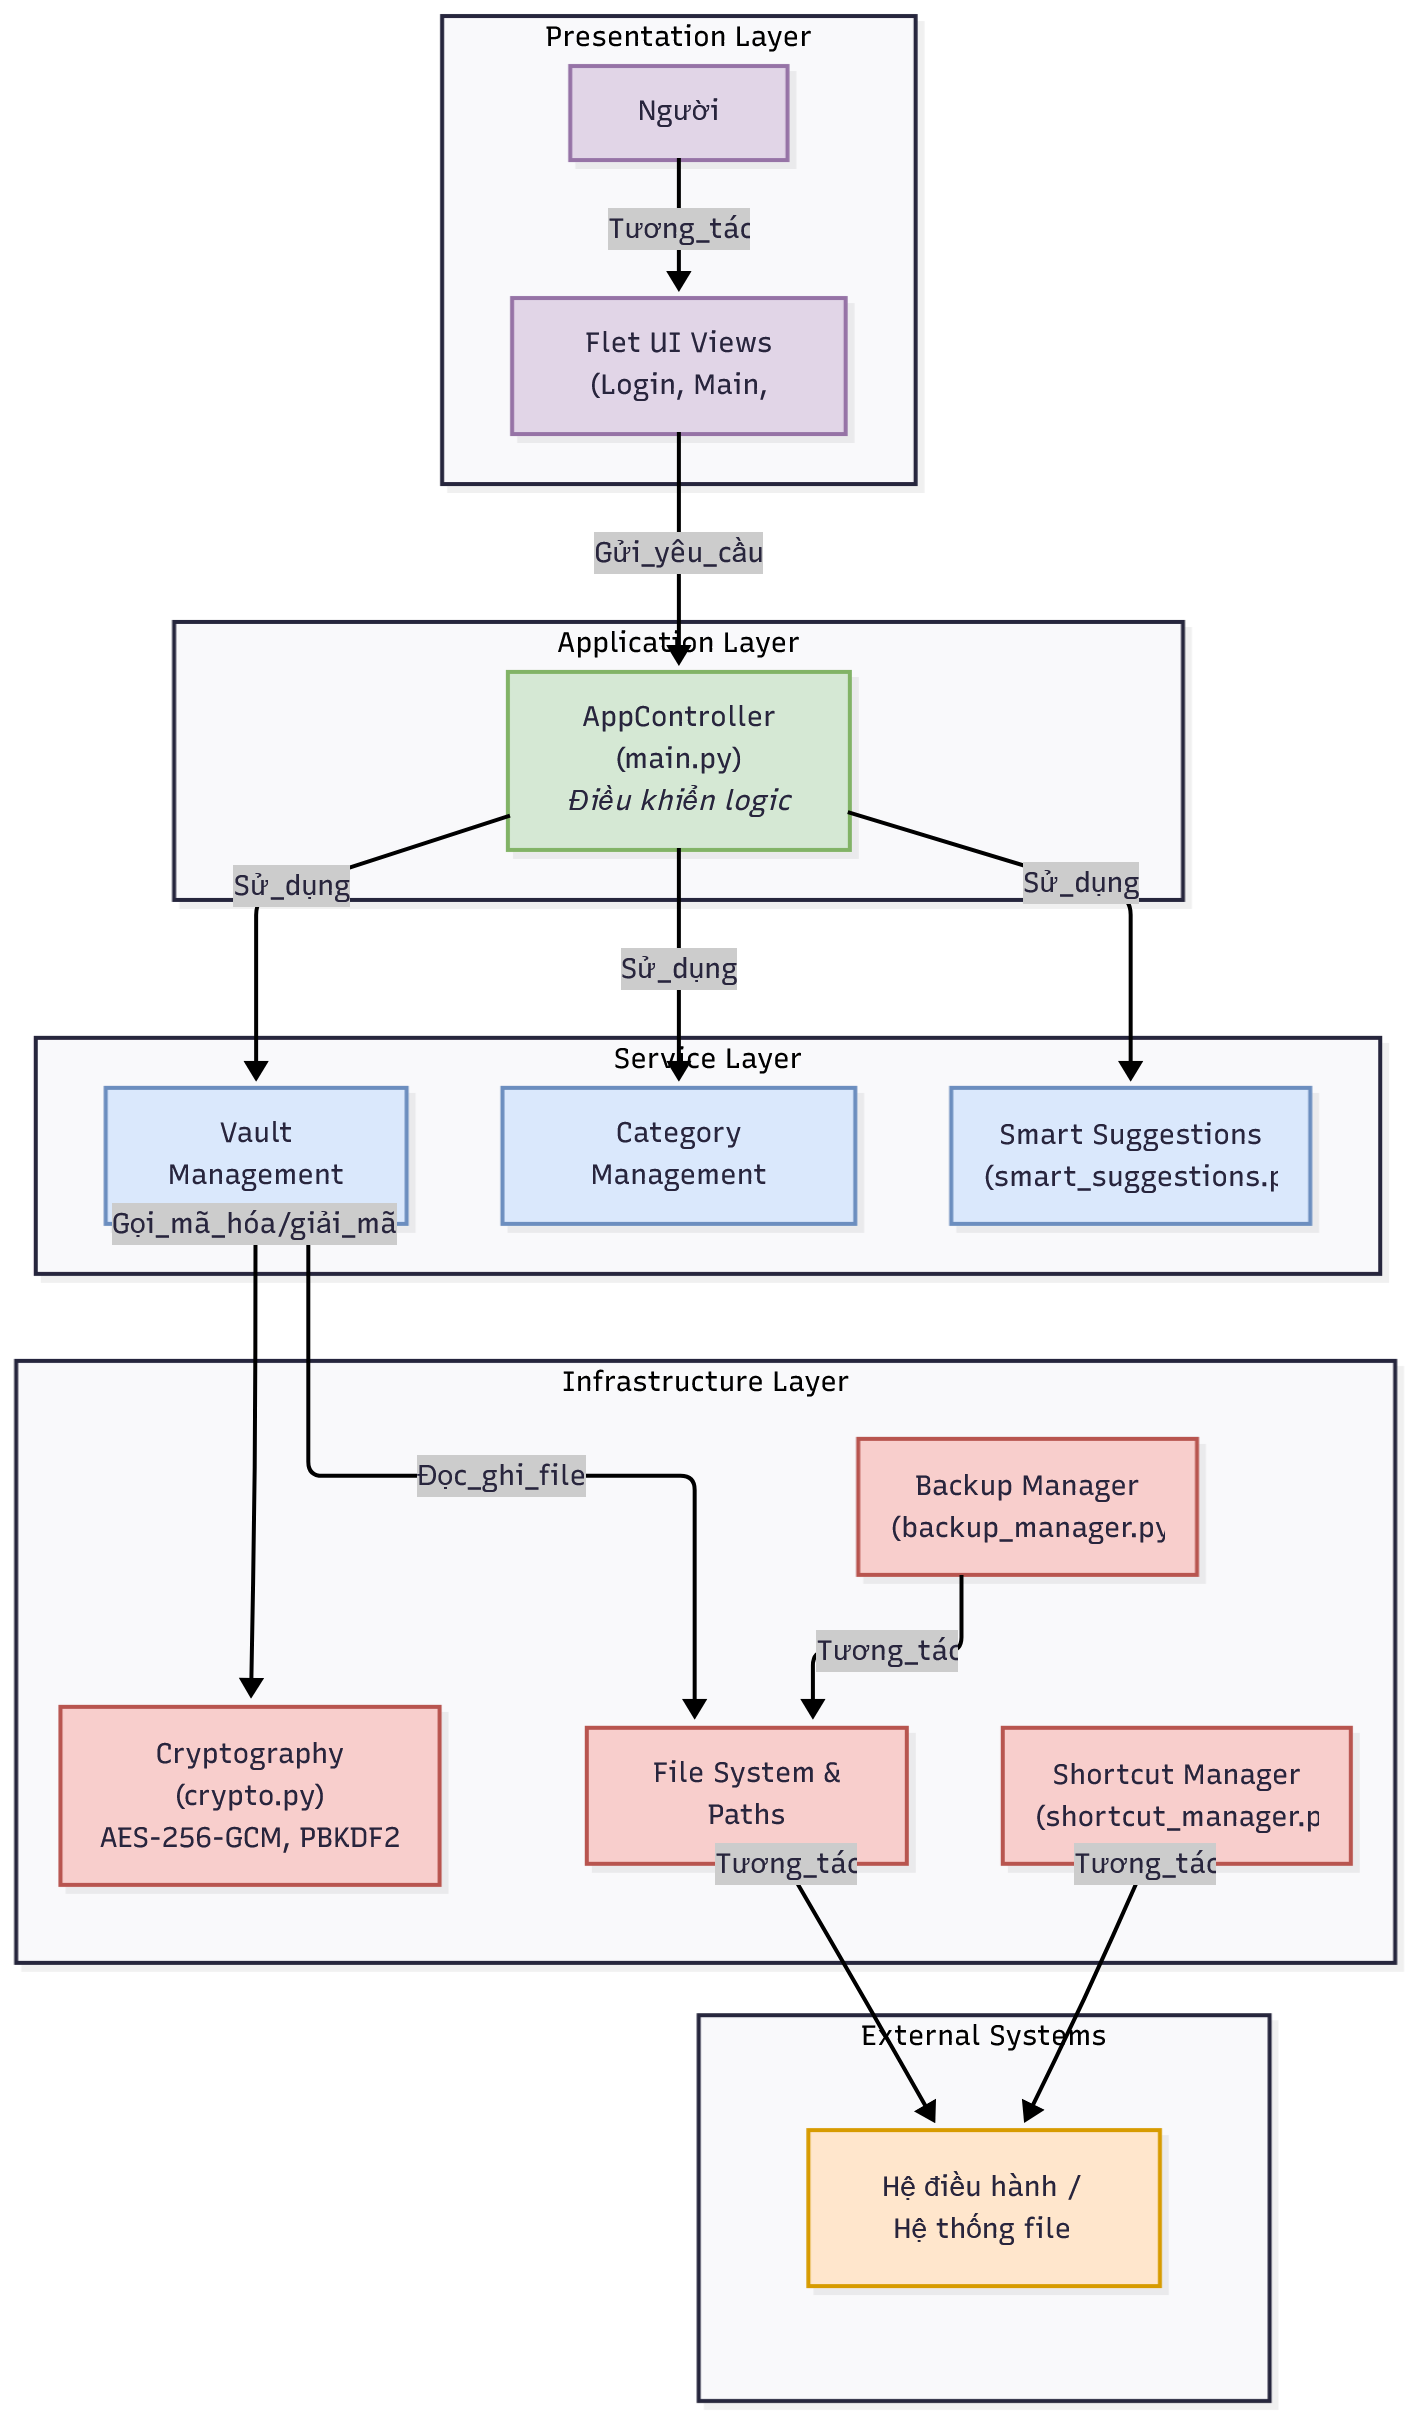
\includegraphics[width=0.8\textwidth]{images/architecture_diagram.png}
    \caption{Kiến trúc tổng quan của AuraCrypt}
    \label{fig:architecture_diagram}
\end{figure}
\textbf{Các lớp chính:}
\begin{itemize}
    \item \textbf{Presentation Layer (Lớp giao diện):} Xử lý các tương tác với người dùng thông qua Flet UI. Bao gồm các view (login, main vault, settings).
    \item \textbf{Application Layer (Lớp ứng dụng):} Chứa logic điều khiển chính của ứng dụng, tương tác với các lớp dưới để thực hiện các yêu cầu của người dùng.
    \item \textbf{Service Layer (Lớp dịch vụ):} Cung cấp các dịch vụ cốt lõi như quản lý vault, tạo mật khẩu, quản lý danh mục.
    \item \textbf{Infrastructure Layer (Lớp hạ tầng):} Bao gồm các module xử lý mã hóa, đọc/ghi file, sao lưu và các tương tác với hệ điều hành (ví dụ: tạo shortcut).
\end{itemize}

\section{Thiết kế cơ sở dữ liệu (Cấu trúc Vault)}
Dữ liệu mật khẩu được lưu trữ dưới dạng một file JSON đã mã hóa.
\begin{lstlisting}[caption=Cấu trúc dữ liệu vault mã hóa]
{
    "salt": "base64_encoded_salt",
    "nonce": "base64_encoded_nonce",
    "ciphertext": "base64_encoded_encrypted_data"
}
\end{lstlisting}
Trong đó, `ciphertext` chứa một đối tượng JSON đã mã hóa với cấu trúc sau:
\begin{lstlisting}[caption=Cấu trúc dữ liệu nội dung vault (chưa mã hóa)]
{
    "master_key_fingerprint": "hash_of_derived_key",
    "entries": [
        {
            "id": "uuid",
            "service": "Tên dịch vụ",
            "username": "Tên người dùng",
            "password": "Mật khẩu",
            "url": "URL liên quan",
            "category": "Danh mục",
            "notes": "Ghi chú",
            "created_at": "timestamp",
            "updated_at": "timestamp"
        }
    ],
    "categories": [
        "Danh mục 1",
        "Danh mục 2"
    ],
    "settings": {
        "auto_lock_timeout": 900,
        "clipboard_clear_delay": 15
    }
}
\end{lstlisting}
\subsection{Quản lý dữ liệu sao lưu}
Các bản sao lưu được lưu trong thư mục \texttt{backups} dưới dạng \texttt{vault\_YYYYMMDD\_HHMMSS.bak}.

\section{Thiết kế giao diện người dùng (UI/UX)}
Giao diện người dùng được thiết kế dựa trên nguyên tắc tối giản, hiện đại và dễ sử dụng.
\begin{itemize}
    \item \textbf{Màn hình Đăng nhập/Thiết lập:} Đơn giản, rõ ràng, hướng dẫn người dùng thiết lập mật khẩu chủ lần đầu.
    \item \textbf{Màn hình chính (Vault):} Hiển thị danh sách mật khẩu, thanh tìm kiếm, bộ lọc danh mục và các nút chức năng (thêm, sửa, xóa).
    \item \textbf{Form thêm/sửa mật khẩu:} Các trường nhập liệu rõ ràng, tích hợp nút tạo mật khẩu mạnh.
\end{itemize}

\begin{figure}[H]
    \centering
    % TODO 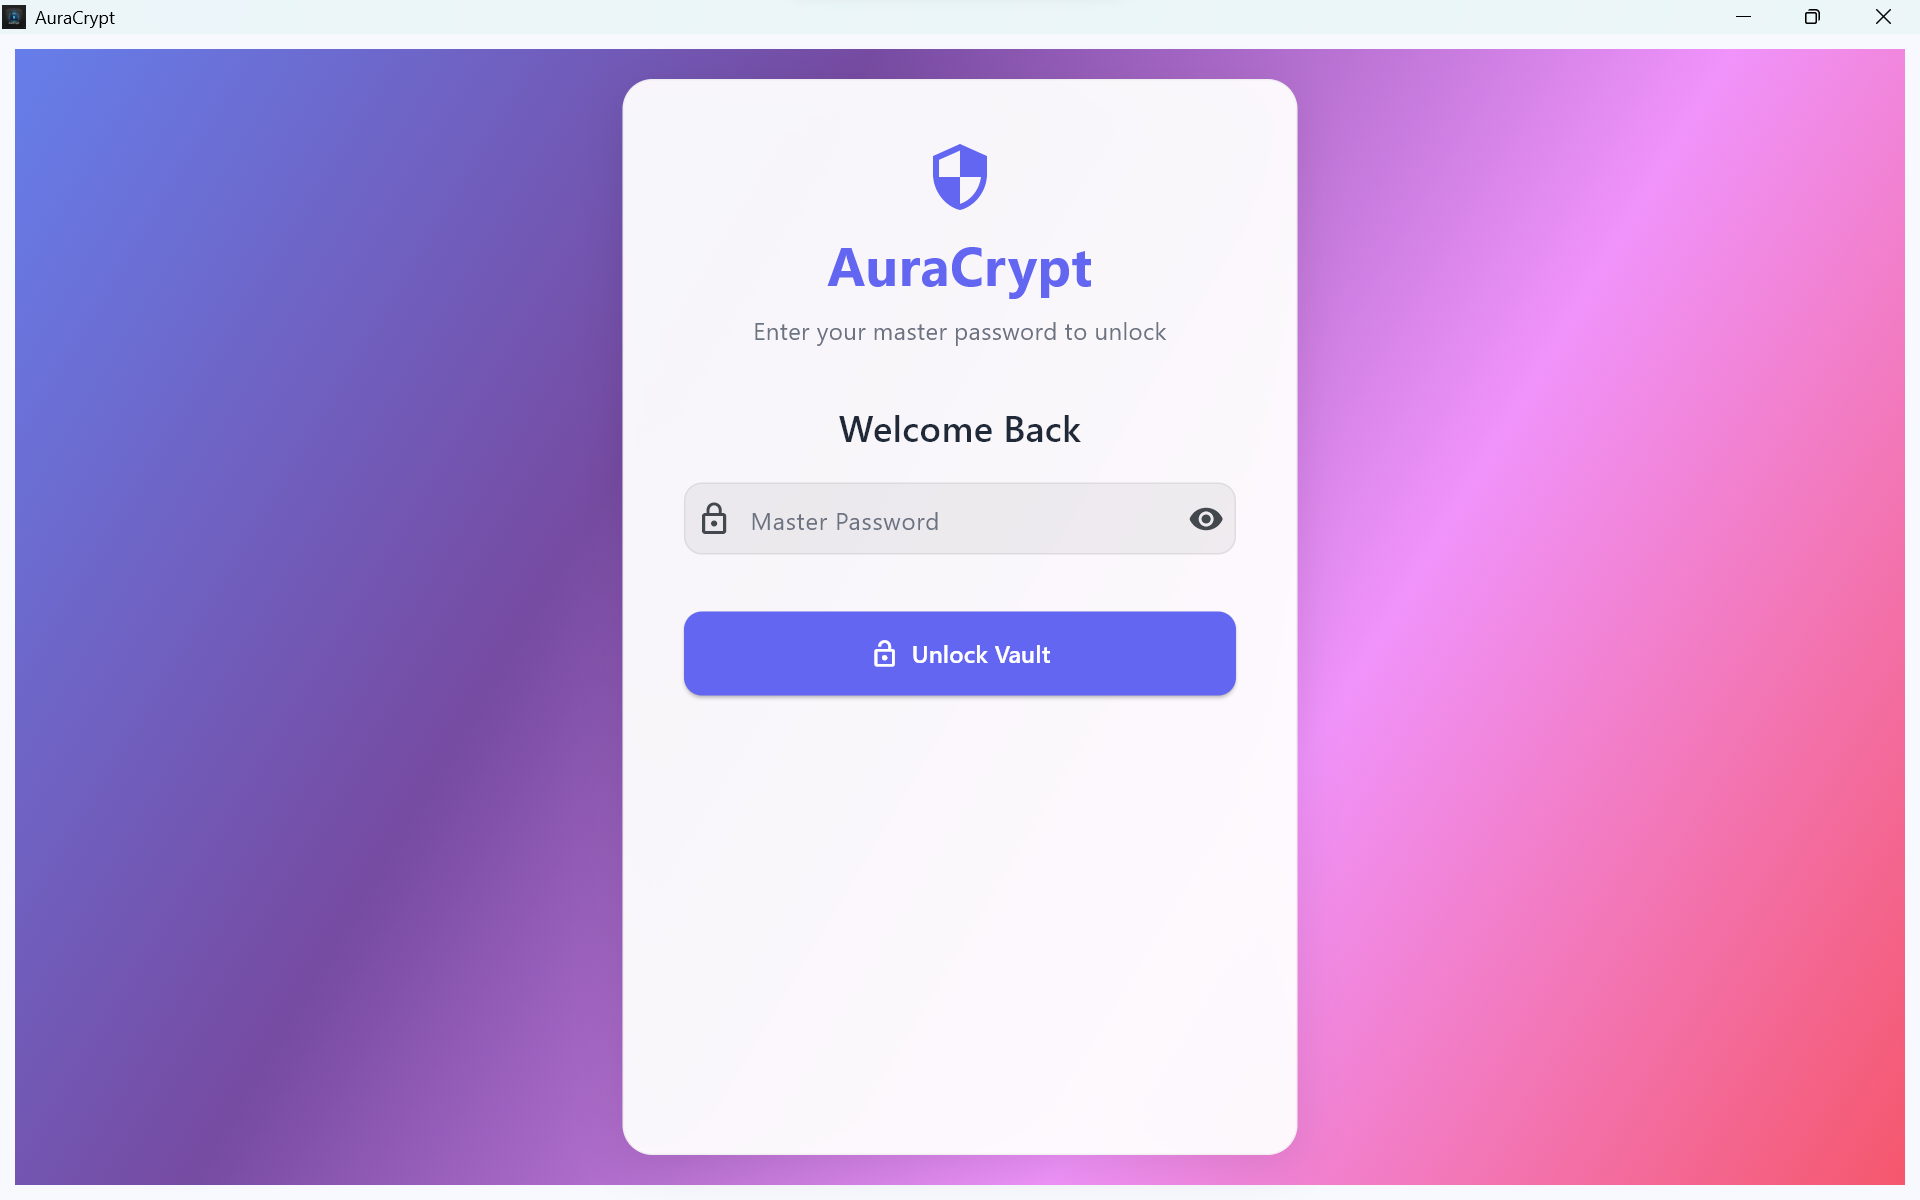
\includegraphics[width=0.7\textwidth]{images/mock_login_screen.png}
    \caption{Thiết kế giao diện màn hình Đăng nhập}
    \label{fig:login_screen}
\end{figure}

\begin{figure}[H]
    \centering
    % TODO 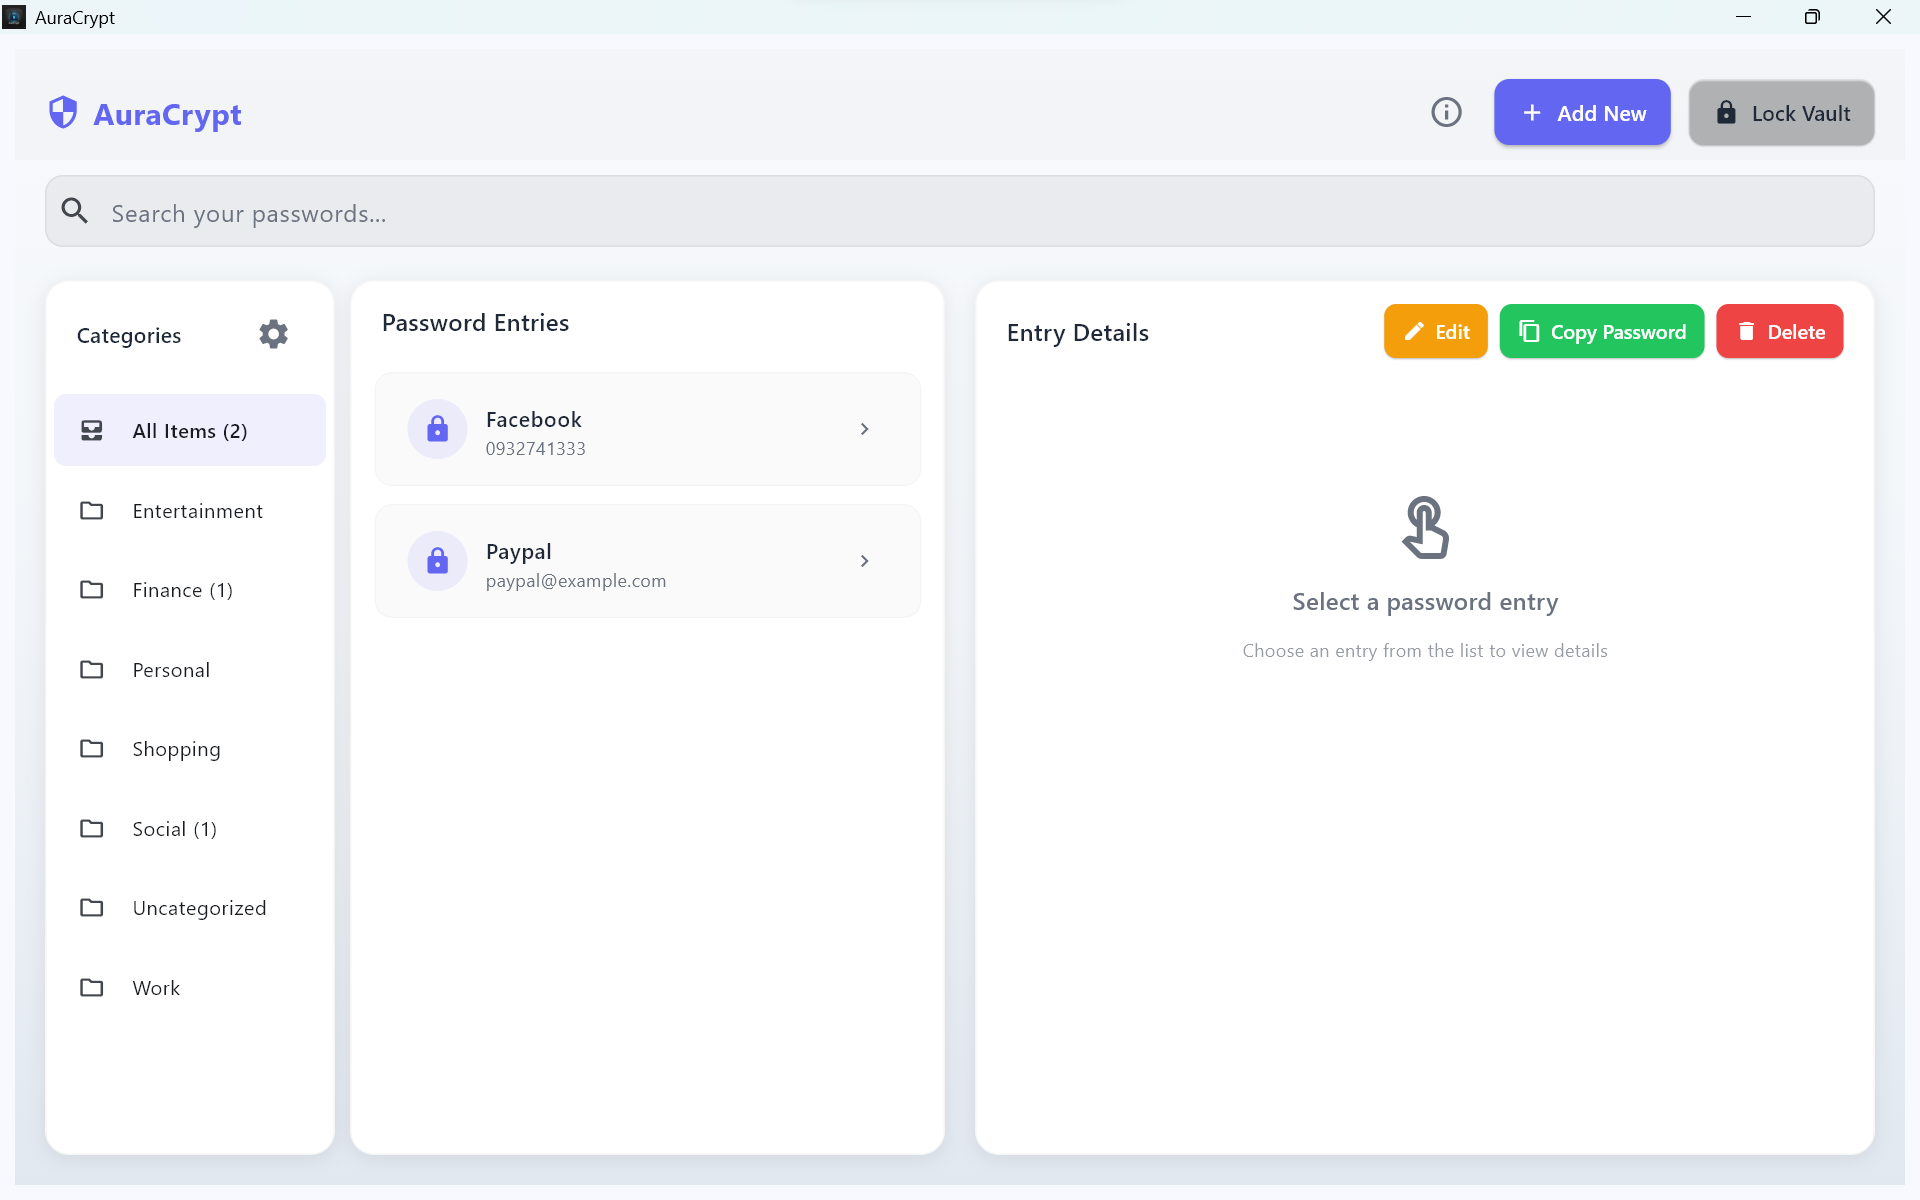
\includegraphics[width=0.7\textwidth]{images/mock_main_screen.png}
    \caption{Thiết kế giao diện màn hình chính}
    \label{fig:main_screen}
\end{figure}
\newpage
\chapter{TRIỂN KHAI VÀ THỬ NGHIỆM}

\section{Môi trường phát triển và công cụ}
\begin{itemize}
    \item \textbf{Hệ điều hành:} Windows 10/11
    \item \textbf{Ngôn ngữ lập trình:} Python 3.10+
    \item \textbf{Framework UI:} Flet 0.20+
    \item \textbf{Môi trường ảo:} `venv`
    \item \textbf{Công cụ đóng gói:} `PyInstaller` (sử dụng thông qua `flet pack`)
    \item \textbf{IDE:} Visual Studio Code
\end{itemize}

\section{Triển khai các chức năng chính}
\subsection{Module mã hóa (`crypto.py`)}
Module này chứa các hàm để thực hiện mã hóa AES-256-GCM, tạo khóa từ mật khẩu chủ bằng PBKDF2, và quản lý salt/nonce.
\lstinputlisting[language=Python, caption=Trích đoạn code mã hóa AES-256-GCM]{core/crypto.py}

\subsection{Module Vault (`vault.py`)}
Module `vault.py` quản lý việc đọc, ghi, mã hóa và giải mã toàn bộ dữ liệu vault. Nó tương tác với `crypto.py` để bảo mật dữ liệu.
\lstinputlisting[language=Python, caption=Trích đoạn code quản lý Vault]{core/vault.py}

\subsection{Quản lý Desktop Shortcut (Windows)}
Tính năng này được triển khai trong `utils/shortcut\_manager.py`, sử dụng thư viện `pywin32` và `winshell` để tương tác với Windows API. Shortcut được tạo tự động khi ứng dụng chạy lần đầu.
\lstinputlisting[language=Python, caption=Trích đoạn code tạo shortcut tự động]{utils/shortcut_manager.py}

\subsection{Giao diện người dùng với Flet}
Flet được sử dụng để xây dựng các thành phần giao diện một cách phản ứng (reactive). Mỗi màn hình (View) được thiết kế là một lớp riêng biệt.
\lstinputlisting[language=Python, caption=Trích đoạn code giao diện màn hình đăng nhập (`ui/login\_view.py`)]{ui/login\_view.py}

\section{Thử nghiệm và đánh giá}
\subsection{Thử nghiệm chức năng}
Tôi đã thực hiện thử nghiệm chức năng cho từng tính năng của ứng dụng, bao gồm:
\begin{itemize}
    \item Thêm, sửa, xóa, tìm kiếm mật khẩu.
    \item Tạo mật khẩu ngẫu nhiên với các tiêu chí khác nhau.
    \item Đăng nhập/đăng xuất, tự động khóa ứng dụng.
    \item Sao lưu và phục hồi dữ liệu.
    \item Nhập/xuất dữ liệu.
    \item Tạo shortcut tự động (trên Windows).
\end{itemize}
Tất cả các chức năng đều hoạt động đúng như thiết kế.

\subsection{Thử nghiệm bảo mật}
\begin{itemize}
    \item \textbf{Kiểm tra mã hóa:} Xác nhận rằng dữ liệu lưu trữ không thể đọc được nếu không có mật khẩu chủ.
    \item \textbf{Kiểm tra hiệu suất PBKDF2:} Đánh giá thời gian cần thiết để dẫn xuất khóa, đảm bảo độ trễ hợp lý chống brute-force.
    \item \textbf{Kiểm tra làm sạch bộ nhớ đệm:} Đảm bảo mật khẩu trên clipboard được xóa sau thời gian quy định.
\end{itemize}
Kết quả thử nghiệm cho thấy AuraCrypt đạt được các yêu cầu bảo mật đã đề ra.

\subsection{Thử nghiệm đóng gói ứng dụng}
Ứng dụng đã được đóng gói thành công thành tệp `.exe` cho Windows, đảm bảo khả năng chạy độc lập và tạo shortcut tự động với icon chính xác.
\begin{figure}[H]
    \centering
    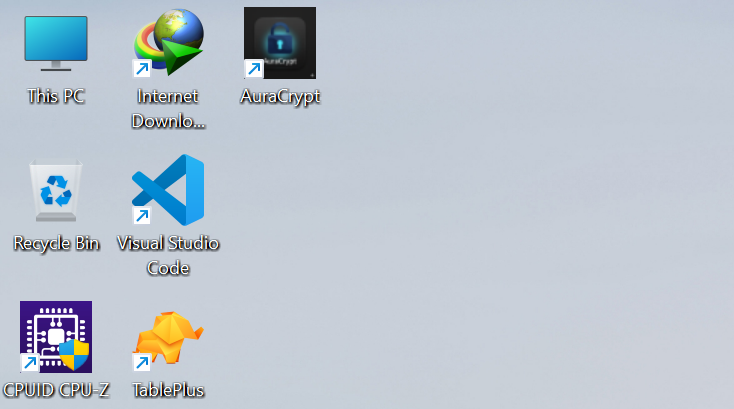
\includegraphics[width=0.6\textwidth]{images/desktop_shortcut_final.png}
    \caption{Shortcut AuraCrypt trên desktop Windows}
    \label{fig:desktop_shortcut}
\end{figure}
\newpage
\chapter{KẾT LUẬN VÀ HƯỚNG PHÁT TRIỂN}

\section{Kết luận}
Đồ án "Phần mềm quản lý mật khẩu an toàn AuraCrypt" đã hoàn thành các mục tiêu đề ra. Tôi đã thành công trong việc thiết kế và triển khai một ứng dụng quản lý mật khẩu an toàn, dễ sử dụng, tích hợp các tính năng bảo mật và tiện ích cần thiết. AuraCrypt cung cấp một giải pháp đáng tin cậy để người dùng bảo vệ thông tin đăng nhập quan trọng của mình.

Những điểm nổi bật của đồ án bao gồm:
\begin{itemize}
    \item Hệ thống mã hóa mạnh mẽ với AES-256-GCM và PBKDF2.
    \item Giao diện người dùng trực quan, thân thiện.
    \item Các tính năng tiện ích như tạo mật khẩu mạnh, quản lý danh mục, sao lưu tự động.
    \item Khả năng đóng gói thành ứng dụng độc lập trên Windows, tự động tạo shortcut.
\end{itemize}
Trong quá trình thực hiện, tôi đã học hỏi được nhiều kiến thức quý báu về mật mã học, kiến trúc phần mềm và quy trình phát triển ứng dụng.

\section{Hạn chế}
Mặc dù đã đạt được nhiều thành công, đồ án vẫn còn một số hạn chế:
\begin{itemize}
    \item \textbf{Chưa hỗ trợ đa nền tảng hoàn chỉnh:} Hiện tại chỉ tập trung tối ưu cho Windows, chưa thử nghiệm đầy đủ trên macOS hoặc Linux với các tính năng đặc thù (ví dụ: tạo shortcut).
    \item \textbf{Chưa tích hợp tự động điền/đăng nhập:} Người dùng vẫn phải sao chép/dán mật khẩu thủ công.
    \item \textbf{Chưa có tính năng đồng bộ hóa:} Dữ liệu chỉ được lưu trữ cục bộ, chưa có cơ chế đồng bộ hóa an toàn giữa các thiết bị.
    \item \textbf{Giao diện cơ bản:} Mặc dù thân thiện, giao diện vẫn có thể được cải thiện để hiện đại và linh hoạt hơn.
\item \textbf{Xử lý ngoại lệ:} Một số trường hợp ngoại lệ hiếm gặp có thể chưa được xử lý tối ưu.
\end{itemize}

\section{Hướng phát triển trong tương lai}
Để cải thiện và mở rộng AuraCrypt, tôi đề xuất các hướng phát triển sau:
\begin{itemize}
    \item \textbf{Tích hợp tính năng tự động điền (Autofill):} Phát triển tiện ích mở rộng trình duyệt hoặc tính năng tự động điền vào các trường đăng nhập trên website.
    \item \textbf{Đồng bộ hóa dữ liệu an toàn:} Nghiên cứu và triển khai cơ chế đồng bộ hóa dữ liệu mã hóa giữa các thiết bị thông qua các dịch vụ đám mây (ví dụ: Google Drive, Dropbox) với bảo mật từ đầu đến cuối (end-to-end encryption).
    \item \textbf{Hỗ trợ đa nền tảng tốt hơn:} Tối ưu hóa cho macOS và Linux, bao gồm cả các tính năng đặc thù của từng hệ điều hành.
    \item \textbf{Xác thực đa yếu tố (MFA):} Tích hợp các phương pháp xác thực thứ cấp (ví dụ: sinh trắc học, TOTP) để tăng cường bảo mật.
    \item \textbf{Cải thiện UI/UX:} Nâng cấp giao diện người dùng, bổ sung thêm các tùy chỉnh và chủ đề (themes) để cá nhân hóa trải nghiệm.
    \item \textbf{Kiểm tra bảo mật chuyên sâu:} Thực hiện các cuộc kiểm tra thâm nhập (penetration testing) và đánh giá lỗ hổng bảo mật chuyên nghiệp.
\end{itemize}

Hy vọng đồ án này sẽ là nền tảng vững chắc cho các nghiên cứu và phát triển tiếp theo trong lĩnh vực quản lý mật khẩu và bảo mật thông tin.
\newpage

% --- PHỤ LỤC (Nếu có) ---
% \appendix % Bắt đầu phần phụ lục
% \input{phuluc_a}
% \input{phuluc_b}

% --- TÀI LIỆU THAM KHẢO ---
% \nocite{*} % Để hiển thị tất cả các mục trong references.bib ngay cả khi không được trích dẫn
% \printbibliography % Nếu dùng biblatex
% Nếu dùng bibtex thủ công:
% \bibliographystyle{plain}
% \bibliography{references}

\end{document}